\documentclass[aspectratio=169,10pt]{beamer}

\usetheme{Madrid}
\usecolortheme{default}
\setbeamertemplate{navigation symbols}{}
\setbeamertemplate{footline}[frame number]

\usepackage[T1]{fontenc}
\usepackage[utf8]{inputenc}
\usepackage{booktabs}
\usepackage{graphicx}
\usepackage{array}
\usepackage{xcolor}

\graphicspath{{outputs/}}

\definecolor{deepblue}{RGB}{31,80,126}
\definecolor{riskred}{RGB}{190,55,55}
\definecolor{safegreen}{RGB}{45,125,85}
\setbeamercolor{title}{fg=deepblue}
\setbeamercolor{frametitle}{fg=white,bg=deepblue}
\setbeamercolor{structure}{fg=deepblue}

\title[IFCS Financial Distress]{Profiling and Predicting Financial Distress in Italian SMEs}
\subtitle{IFCS 2026 Data Challenge}
\author{}
\date{}

\newcommand{\pct}[1]{#1\%}
\newcommand{\keuro}{kEUR}

\begin{document}

\begin{frame}
  \titlepage
  \vspace{-0.7cm}
  \begin{center}
    \small FY2023 financial statements, unsupervised profiles, and supervised distress prediction
  \end{center}
\end{frame}

\begin{frame}{Problem and Data}
  \begin{columns}[T,totalwidth=\textwidth]
    \begin{column}{0.52\textwidth}
      \textbf{Objective}
      \begin{itemize}
        \item Profile SMEs using financial characteristics.
        \item Predict \texttt{Financial distress}.
        \item Produce interpretable evidence for lenders, policy makers, and firms.
      \end{itemize}

      \vspace{0.25cm}
      \textbf{Dataset}
      \begin{itemize}
        \item 13,956 Italian SMEs.
        \item 14 feature columns plus binary target.
        \item 108 provinces, 306 sectors, 268 ATECO codes.
      \end{itemize}
    \end{column}

    \begin{column}{0.42\textwidth}
      \begin{block}{Target imbalance}
        \centering
        \begin{tabular}{lr}
          \toprule
          Class & Firms \\
          \midrule
          Not distressed & 12,451 \\
          Distressed & 1,505 \\
          \midrule
          Distress rate & \pct{10.78} \\
          \bottomrule
        \end{tabular}
      \end{block}

      \vspace{0.15cm}
      \small
      Because the positive class is rare, model quality is judged with F1,
      balanced accuracy, recall, precision, ROC-AUC, and average precision.
    \end{column}
  \end{columns}
\end{frame}

\begin{frame}{Clustering Design}
  \begin{columns}[T,totalwidth=\textwidth]
    \begin{column}{0.48\textwidth}
      \textbf{Principle}
      \begin{itemize}
        \item Cluster on financial behavior only.
        \item Exclude \texttt{Financial distress}, \texttt{Province}, \texttt{sector}, and \texttt{Ateco}.
        \item Use geography and sector only after clustering, for interpretation.
      \end{itemize}

      \vspace{0.15cm}
      \textbf{Preprocessing}
      \begin{itemize}
        \item Signed logs for skewed monetary variables.
        \item Margins and per-employee productivity ratios.
        \item Debt-pressure and cash-flow ratios.
        \item Winsorization at 0.5th and 99.5th percentiles.
        \item Median imputation and robust scaling.
      \end{itemize}
    \end{column}

    \begin{column}{0.46\textwidth}
      \begin{block}{Chosen solution}
        \centering
        \Large \textbf{k = 5}

        \vspace{0.2cm}
        \normalsize
        A financially interpretable ladder:
        \begin{enumerate}
          \item resilient cash generators
          \item healthy profitable firms
          \item thin-margin vulnerable firms
          \item debt-burdened break-even firms
          \item loss-making cash-flow distressed firms
        \end{enumerate}
      \end{block}

      \vspace{0.1cm}
      \small
      The k=5 solution is more useful for presentation than the trivial
      two-cluster split between broadly healthy and broadly distressed firms.
    \end{column}
  \end{columns}
\end{frame}

\begin{frame}{Five Financial Profiles}
  \scriptsize
  \begin{tabular}{p{0.32\textwidth}rrrrp{0.26\textwidth}}
    \toprule
    Cluster & Firms & Distress & Net margin & OCF margin & Interpretation \\
    \midrule
    A Resilient high-profit cash generators
      & 2,085 & \pct{0.43} & \pct{15.6} & \pct{19.7}
      & strong profits, strong cash flow, very low financial-expense pressure \\
    B Healthy profitable core SMEs
      & 6,043 & \pct{2.75} & \pct{4.5} & \pct{7.4}
      & stable middle: profitable, cash-generative, moderate scale \\
    C Thin-margin vulnerable operators
      & 4,745 & \pct{15.68} & \pct{0.7} & \pct{3.2}
      & low margin, lower productivity, more sensitive to shocks \\
    D Debt-burdened break-even firms
      & 174 & \pct{31.61} & \pct{-1.8} & \pct{1.5}
      & near break-even operations with high financial-expense burden \\
    E Loss-making cash-flow distressed firms
      & 909 & \pct{58.42} & \pct{-10.2} & \pct{-6.1}
      & losses and negative operating cash flow dominate \\
    \bottomrule
  \end{tabular}

  \vspace{0.3cm}
  \normalsize
  \textbf{Main interpretation:} distress rises smoothly as profitability,
  productivity, and operating cash flow deteriorate.
\end{frame}

\begin{frame}{Cluster Map: UMAP View}
  \begin{columns}[T,totalwidth=\textwidth]
    \begin{column}{0.68\textwidth}
      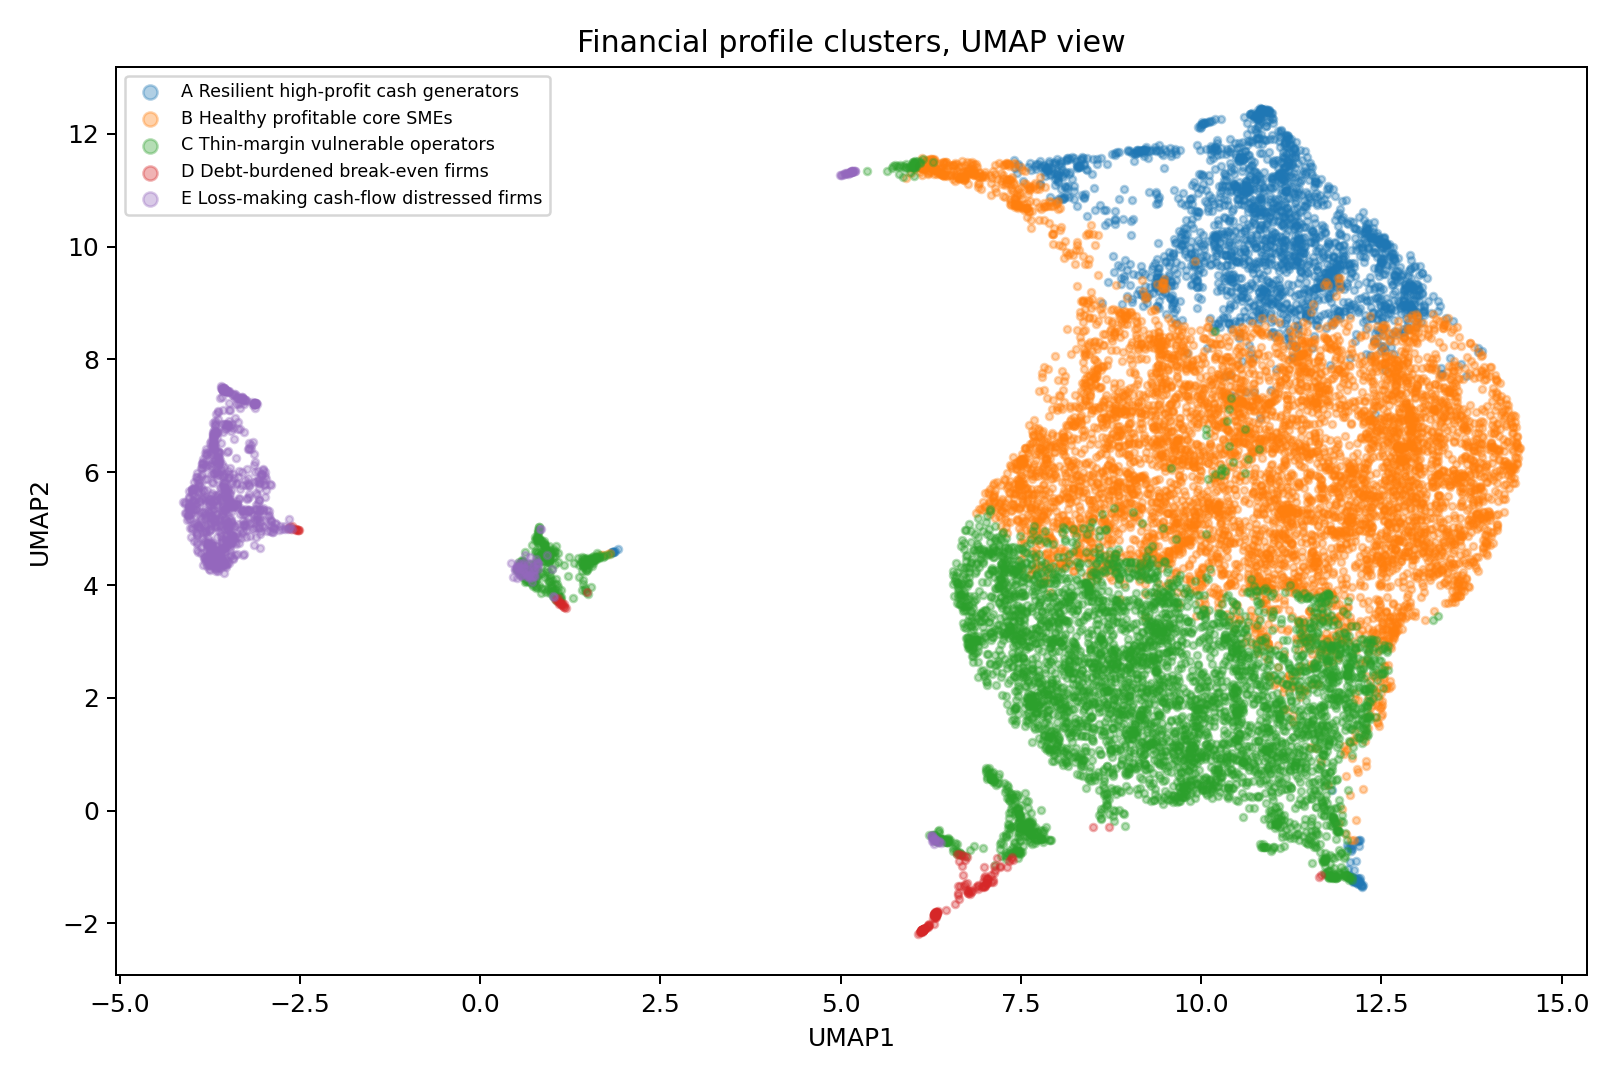
\includegraphics[width=\textwidth]{cluster_umap.png}
    \end{column}
    \begin{column}{0.28\textwidth}
      \textbf{Why this plot matters}
      \begin{itemize}
        \item UMAP projects the same financial feature space used for k-means.
        \item The loss-making profile separates clearly.
        \item Thin-margin and healthy firms form the large operating core.
        \item The small debt-burdened group appears as a narrow transition profile.
      \end{itemize}
    \end{column}
  \end{columns}
\end{frame}

\begin{frame}{Geographic Pattern}
  \begin{columns}[T,totalwidth=\textwidth]
    \begin{column}{0.62\textwidth}
      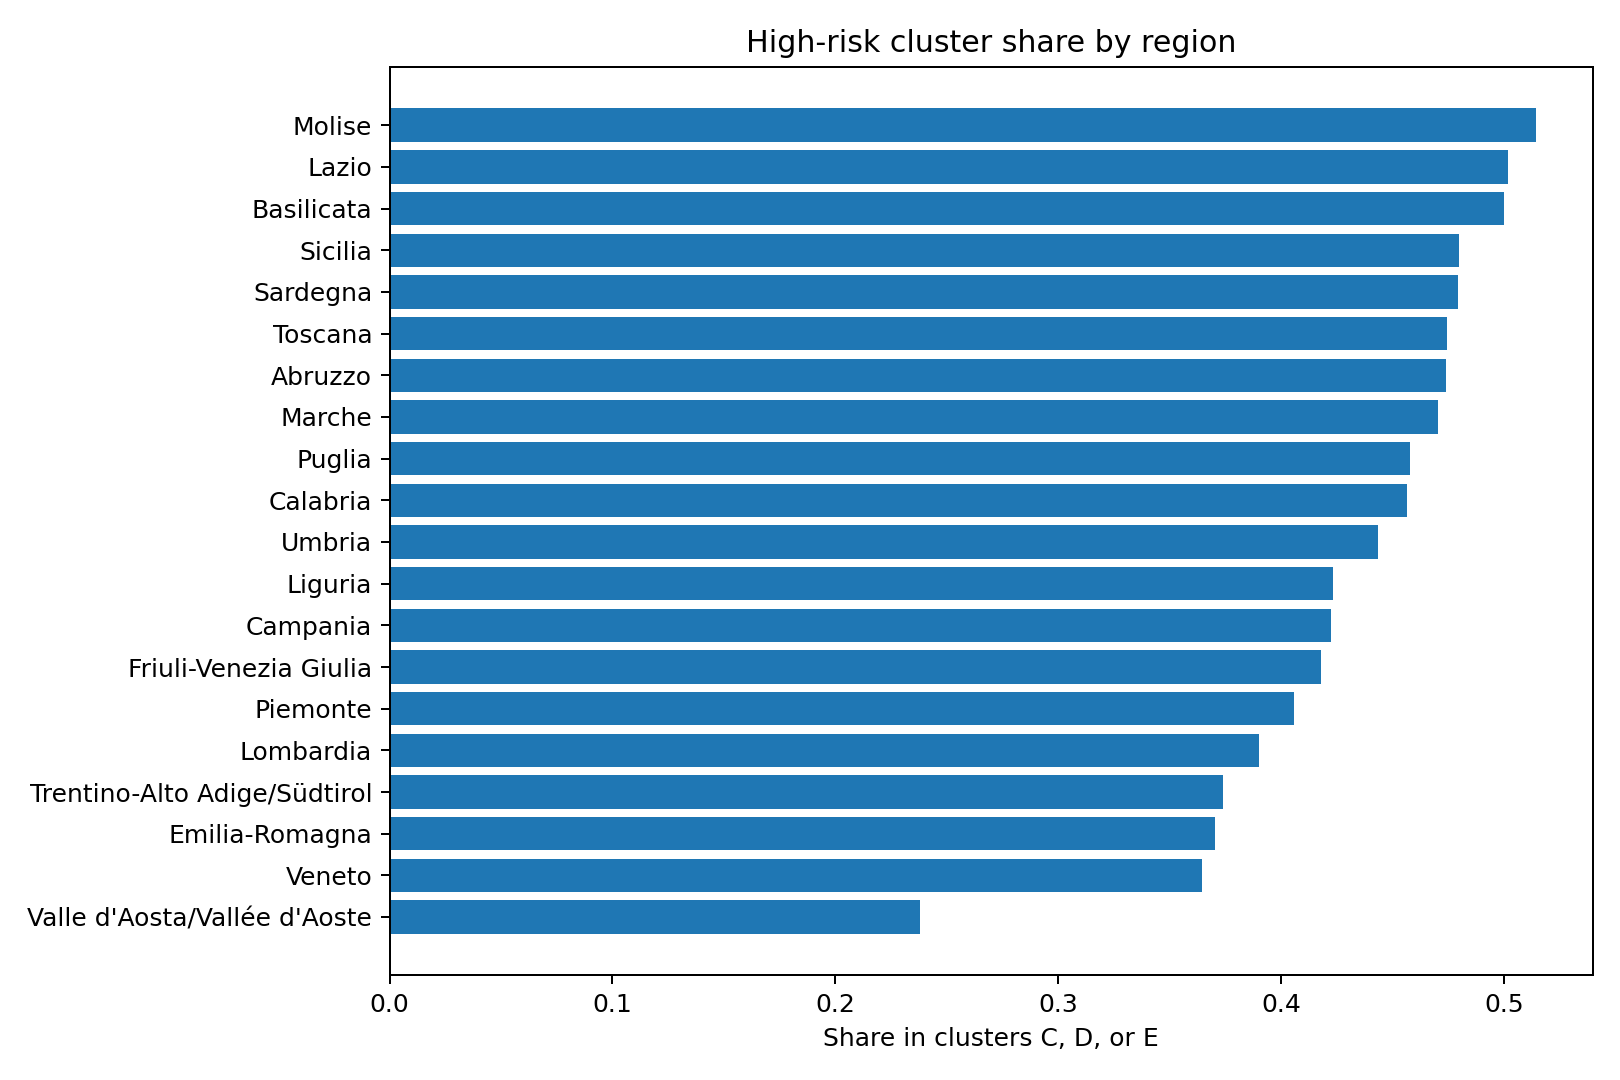
\includegraphics[width=\textwidth]{region_high_risk_cluster_share.png}
    \end{column}
    \begin{column}{0.34\textwidth}
      \textbf{High-risk profiles}
      \begin{itemize}
        \item C: thin-margin vulnerable operators
        \item D: debt-burdened break-even firms
        \item E: loss-making cash-flow distressed firms
      \end{itemize}

      \vspace{0.15cm}
      \textbf{Top shares}
      \begin{tabular}{lr}
        \toprule
        Region & Share \\
        \midrule
        Molise & \pct{51.43} \\
        Lazio & \pct{50.17} \\
        Basilicata & \pct{50.00} \\
        Sicilia & \pct{48.01} \\
        Sardegna & \pct{47.96} \\
        \bottomrule
      \end{tabular}
    \end{column}
  \end{columns}

  \vspace{0.15cm}
  \small
  The chart describes concentration of fragile financial profiles, not a causal
  effect of location.
\end{frame}

\begin{frame}{Prediction Model: Rank Ensemble}
  \begin{columns}[T,totalwidth=\textwidth]
    \begin{column}{0.46\textwidth}
      \textbf{Models}
      \begin{itemize}
        \item ExtraTrees
        \item LightGBM
        \item XGBoost
        \item HistGradientBoosting
        \item CatBoost with native categorical features
      \end{itemize}

      \vspace{0.15cm}
      \textbf{Ensembling}
      \begin{itemize}
        \item Convert each model's OOF scores to ranks.
        \item Average ranks across models.
        \item Threshold the rank ensemble.
      \end{itemize}
    \end{column}

    \begin{column}{0.48\textwidth}
      \begin{block}{Out-of-fold performance}
        \centering
        \begin{tabular}{lr}
          \toprule
          Metric & Value \\
          \midrule
          ROC-AUC & 0.880 \\
          Average precision & 0.522 \\
          Best-F1 threshold & 0.88 \\
          F1 & 0.517 \\
          Precision & 0.512 \\
          Recall & 0.522 \\
          Accuracy & 0.895 \\
          \bottomrule
        \end{tabular}
      \end{block}

      \vspace{0.1cm}
      \small
      If the metric rewards recall or balanced accuracy, the threshold should
      be lowered to roughly 0.70--0.71.
    \end{column}
  \end{columns}
\end{frame}

\begin{frame}{OOF Scores: True Class vs Ensemble Risk}
  \begin{columns}[T,totalwidth=\textwidth]
    \begin{column}{0.67\textwidth}
      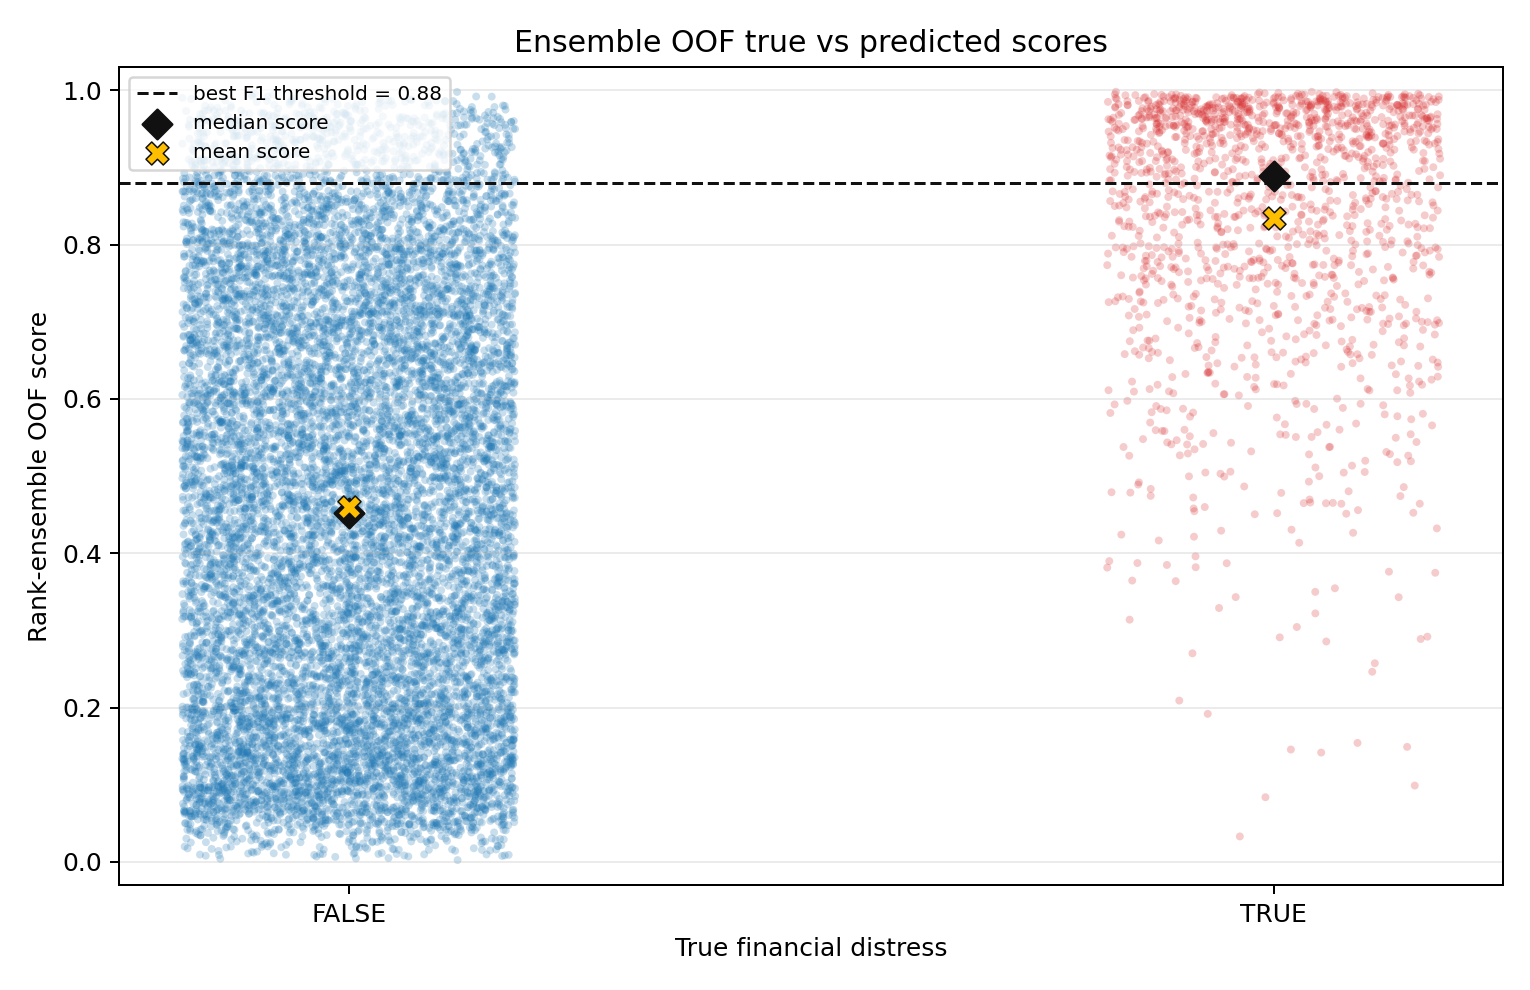
\includegraphics[width=\textwidth]{ensemble_oof_true_predicted.png}
    \end{column}
    \begin{column}{0.29\textwidth}
      \textbf{At threshold 0.88}
      \vspace{0.1cm}

      \begin{tabular}{lr}
        \toprule
        Outcome & Count \\
        \midrule
        True negatives & 11,702 \\
        False positives & 749 \\
        False negatives & 719 \\
        True positives & 786 \\
        \bottomrule
      \end{tabular}

      \vspace{0.25cm}
      \small
      Distressed firms receive much higher ensemble risk scores on average,
      but there is overlap near the decision boundary.
    \end{column}
  \end{columns}
\end{frame}

\begin{frame}{What Drives Predicted Distress?}
  \begin{columns}[T,totalwidth=\textwidth]
    \begin{column}{0.51\textwidth}
      \small
      \begin{tabular}{rl}
        \toprule
        Rank & Feature \\
        \midrule
        1 & net income per employee \\
        2 & sector \\
        3 & cash flow -- net income gap \\
        4 & taxes / operating income \\
        5 & ATECO code \\
        6 & financial expenses / abs. operating income \\
        7 & revenue per employee \\
        8 & province \\
        9 & net income signed log \\
        10 & operating margin \\
        \bottomrule
      \end{tabular}
    \end{column}

    \begin{column}{0.43\textwidth}
      \textbf{Interpretation}
      \begin{itemize}
        \item Distress is primarily a profitability and cash-flow problem.
        \item Sector and ATECO add activity-specific risk.
        \item Province contributes additional geographic signal.
        \item Debt pressure matters relative to operating capacity.
      \end{itemize}
    \end{column}
  \end{columns}
\end{frame}

\begin{frame}{Final Takeaway}
  \begin{block}{The clustering and prediction stories agree}
    Firms move from low-risk to high-risk profiles as margins, cash flow,
    productivity, and debt-service capacity weaken.
  \end{block}

  \vspace{0.25cm}
  \begin{columns}[T,totalwidth=\textwidth]
    \begin{column}{0.47\textwidth}
      \textbf{Interpretation}
      \begin{itemize}
        \item Five clusters provide an economic map of SME vulnerability.
        \item Geography and sector explain where fragile profiles are concentrated.
      \end{itemize}
    \end{column}
    \begin{column}{0.47\textwidth}
      \textbf{Prediction}
      \begin{itemize}
        \item Rank ensemble provides robust OOF risk ordering.
        \item F1 threshold is the default submission choice unless the hidden metric
          rewards recall more strongly.
      \end{itemize}
    \end{column}
  \end{columns}

  \vspace{0.25cm}
  \centering
  \Large \textbf{The model is useful because it is both predictive and explainable.}
\end{frame}

\end{document}
